\begin{sloppypar}
\chapter{Tecnologie impiegate}
\fontsize{12}{19}\selectfont{
In questo capitolo sono descritte in dettaglio le tecnologie utilizzate per la realizzazione dell'applicazione. 
Lo studio di esse ha occupato una parte rilevante del lavoro di tesi in quanto si tratta di tecnologie di nuova generazione, come di seguito elencate:
\vspace{0.2cm}
\begin{enumerate}
    \item  \textbf{Pepper}: robot umanoide progettato e sviluppato dall'azienda \textit{SoftBank Robotics}\texttrademark, specializzata nella progettazione, sviluppo e commercializzazione di robot umanoidi e servizi robotici intelligenti.
\vspace{0.3cm}
\item  \textbf{Choregraphe}: software sviluppato dall'azienda \textit{SoftBank Robotics}\texttrademark, progettato specificamente
per la programmazione e la gestione dei robot umanoidi della
famiglia \textit{NAO}, compresi \textit{NAO} e \textit{Pepper}.
\vspace{0.3cm}
\item \textbf{NAOqi OS}: un sistema operativo sviluppato da\textit{ SoftBank Robotics}\texttrademark, che fornisce
un’interfaccia di programmazione completa e potente, per accedere e
controllare le funzionalità dei robot della famiglia \textit{NAO}.
\end{enumerate}
\begin{figure}[H]
\centering
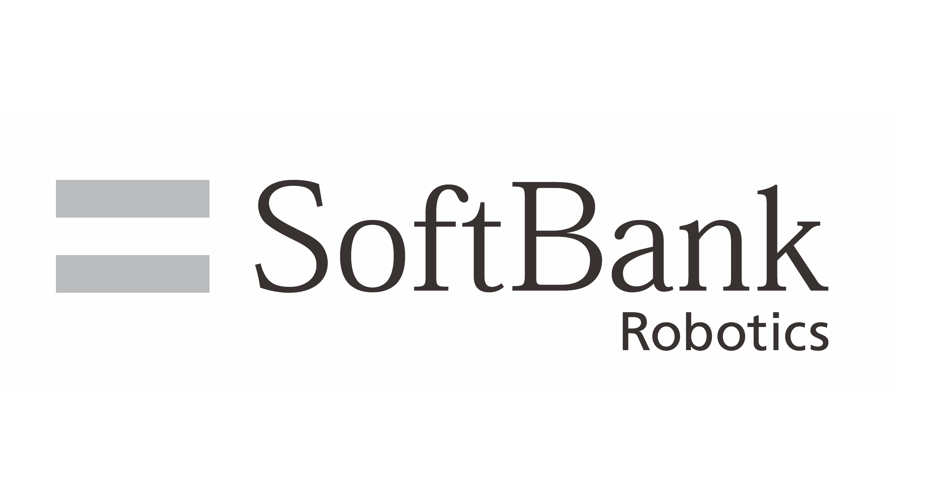
\includegraphics[width=0.65\textwidth]{immagini/softbank.png}
\caption{Logo dell'azienda SoftBank Robotics}
\end{figure}
\vspace{0.4cm}
}
\section{Pepper}
\fontsize{12}{19}\selectfont{Pepper è un robot umanoide progettato e sviluppato dall'azienda SoftBank Robotics\texttrademark,
un’azienda specializzata nella creazione di robot sociali \cite{NAO}. Ha un’altezza di circa 1
metro e 20 cm, un peso di circa 30 kg e presenta un design in grado di conferirgli
sembianze umane. Esso è alimentato da un sistema operativo basato su \textit{Linux} e utilizza una
combinazione di software proprietari e applicazioni sviluppate da terze parti per
fornire una vasta gamma di funzionalità. 
È stato progettato per svolgere compiti
come l’assistenza all’utente, la presentazione di informazioni, l’intrattenimento
e l’interazione sociale. 
\newline
L’obiettivo principale del suo utilizzo è quello di creare
connessione emotiva con l’utente, offrendo un’esperienza coinvolgente e personalizzata.
\vspace{1cm}
\begin{figure}[H]
\centering
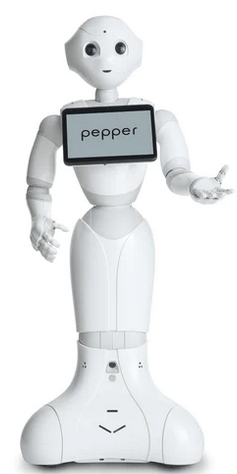
\includegraphics[width=0.33\textwidth]{immagini/pepper1.png}
\caption{Robot umanoide Pepper}
\end{figure}
\vspace{1cm}
Pepper è costituito da un sistema a tre strati.
\newline
La testa contiene tutti i sensori e i componenti di elaborazione dei dati, compresi microfoni, telecamere, sensori di prossimità e un processore \textit{Intel \textsuperscript{\textregistered} Atom\texttrademark}. 
\newline
Il torace ospita il computer principale, che include una \textit{CPU}, una \textit{GPU}, memoria \textit{RAM} e \textit{flash}, nonché connettività \textit{Wi-Fi} e \textit{Ethernet} per consentire il collegamento a Internet e l'accesso a informazioni e servizi basati sul cloud.
\newline
La base contiene le ruote per la mobilità del robot, la batteria per l'alimentazione e sonar per l'individuazione di ostacoli durante lo spostamento del robot.
\newline
L'androide è equipaggiato con un vasto assortimento di sensori,
tra cui telecamere, microfoni direzionali, sensori di prossimità e sensori tattili, che
gli consentono di percepire l’ambiente circostante e interagire in modo intelligente
con le persone. 
\newline
Questi vengono elencati ed analizzati di seguito:
\vspace{0.3cm}
\begin{itemize}
   \item \textbf{Sensori di contatto}: situati nelle mani e nelle dita, consentono a Pepper di rilevare il tocco e le interazioni fisiche.
   \vspace{0.3cm}
   \item \textbf{Sensori di prossimità}: posizionati nel petto, rilevano la presenza di oggetti o persone nelle vicinanze.
   \vspace{0.3cm}
   \item \textbf{Sensori a infrarossi}: consentono a Pepper di misurare la distanza dagli oggetti e di eluderli per evitare collisioni.
   \vspace{0.25cm}
   \item \textbf{Microfoni}: permettono al robot di rilevare e registrare i suoni ambientali.
   \vspace{0.3cm}
   \item \textbf{Telecamere}: Pepper ha telecamere ad alta definizione posizionate nella testa e nel petto per riconoscere i volti, rilevare le espressioni facciali e percepire l'ambiente visivo.
   \vspace{0.3cm}
\end{itemize}
Il robot utilizza una combinazione di ruote e giunti per il movimento. Ha ruote omnidirezionali nella base che gli consentono di ruotare in ogni direzione in modo fluido. Inoltre l'automa è equipaggiato con un sistema di riconoscimento vocale avanzato che gli consente di comprendere e rispondere a comandi vocali in diverse lingue. Ancora, è in grado di analizzare il linguaggio naturale utilizzando algoritmi di elaborazione del linguaggio e di generare risposte coerenti.
\newline
Pepper utilizza il framework NAOqi, basato su Linux, che fornisce un'ampia gamma di API e strumenti per gli sviluppatori per creare applicazioni personalizzate e ampliare le capacità del robot.\newline
Gli sviluppatori possono creare moduli comportamentali, implementare algoritmi di visione artificiale, elaborare dati sensoriali e personalizzare l'interazione con l'utente.
Infine, Pepper presenta un display touch da 10,1 pollici montato sul petto. Questo schermo viene utilizzato per visualizzare informazioni e comunicare con l'utente tramite interfacce personalizzate.
\newline
In conclusione, la sua versatilità, la sua tecnologia innovativa e la capacità
di interazione \textit{user-friendly} lo hanno reso sicuramente un prezioso e interessante
strumento, offrendo opportunità
di apprendimento e di sperimentazione nelle nuove frontiere della robotica e
dell’intelligenza artificiale.
}
\section{Choregraphe}
\fontsize{12}{19}\selectfont{Aldebaran Choregraphe \cite{Aldebaran} è un ambiente di programmazione visuale utilizzato
per creare e gestire comportamenti di robot umanoidi della famiglia NAO, messo
a disposizione dalla SoftBank Robotics. 
\vspace{1cm}
\begin{figure}[H]
\centering
\includegraphics[width=0.5\textwidth]{immagini/choregraphe.png}
\caption{Logo del software Aldebaran Choregraphe}
\end{figure}
\vspace{1cm}



Esso offre un ambiente di sviluppo
basato su un’interfaccia grafica intuitiva, che permette agli sviluppatori di programmare
i robot utilizzando il concetto di "grafi di comportamento". Questi
grafi rappresentano una serie di azioni, movimenti e interazioni che il robot può
eseguire. I comportamenti possono essere creati collegando blocchi funzionali predefiniti,
chiamati \textit{"box"}, tramite linee di connessione che rappresentano il flusso
dell’esecuzione delle azioni del robot.\newline Ogni box rappresenta una specifica azione o una sequenza di azioni che il
robot può compiere, come ad esempio camminare, riconoscere il volto umano o
riprodurre un suono.\newline
Choregraphe fornisce anche una vasta gamma di strumenti per la personalizzazione
dei comportamenti dei robot. Infatti tramite l’utilizzo di script Python
all’interno del software, è possibile estendere le funzionalità di base dei box predefiniti o creare nuovi box personalizzati.\newline Sono messi a disposizione dello sviluppatore anche strumenti di simulazione (\textit{virtual robot}) che consentono di testare i comportamenti dei robot senza doverli eseguire fisicamente. Ciò facilita il processo di debugging e di ottimizzazione delle sequenze di azioni sviluppate.
\vspace{1cm}
\begin{figure}[H]
\centering
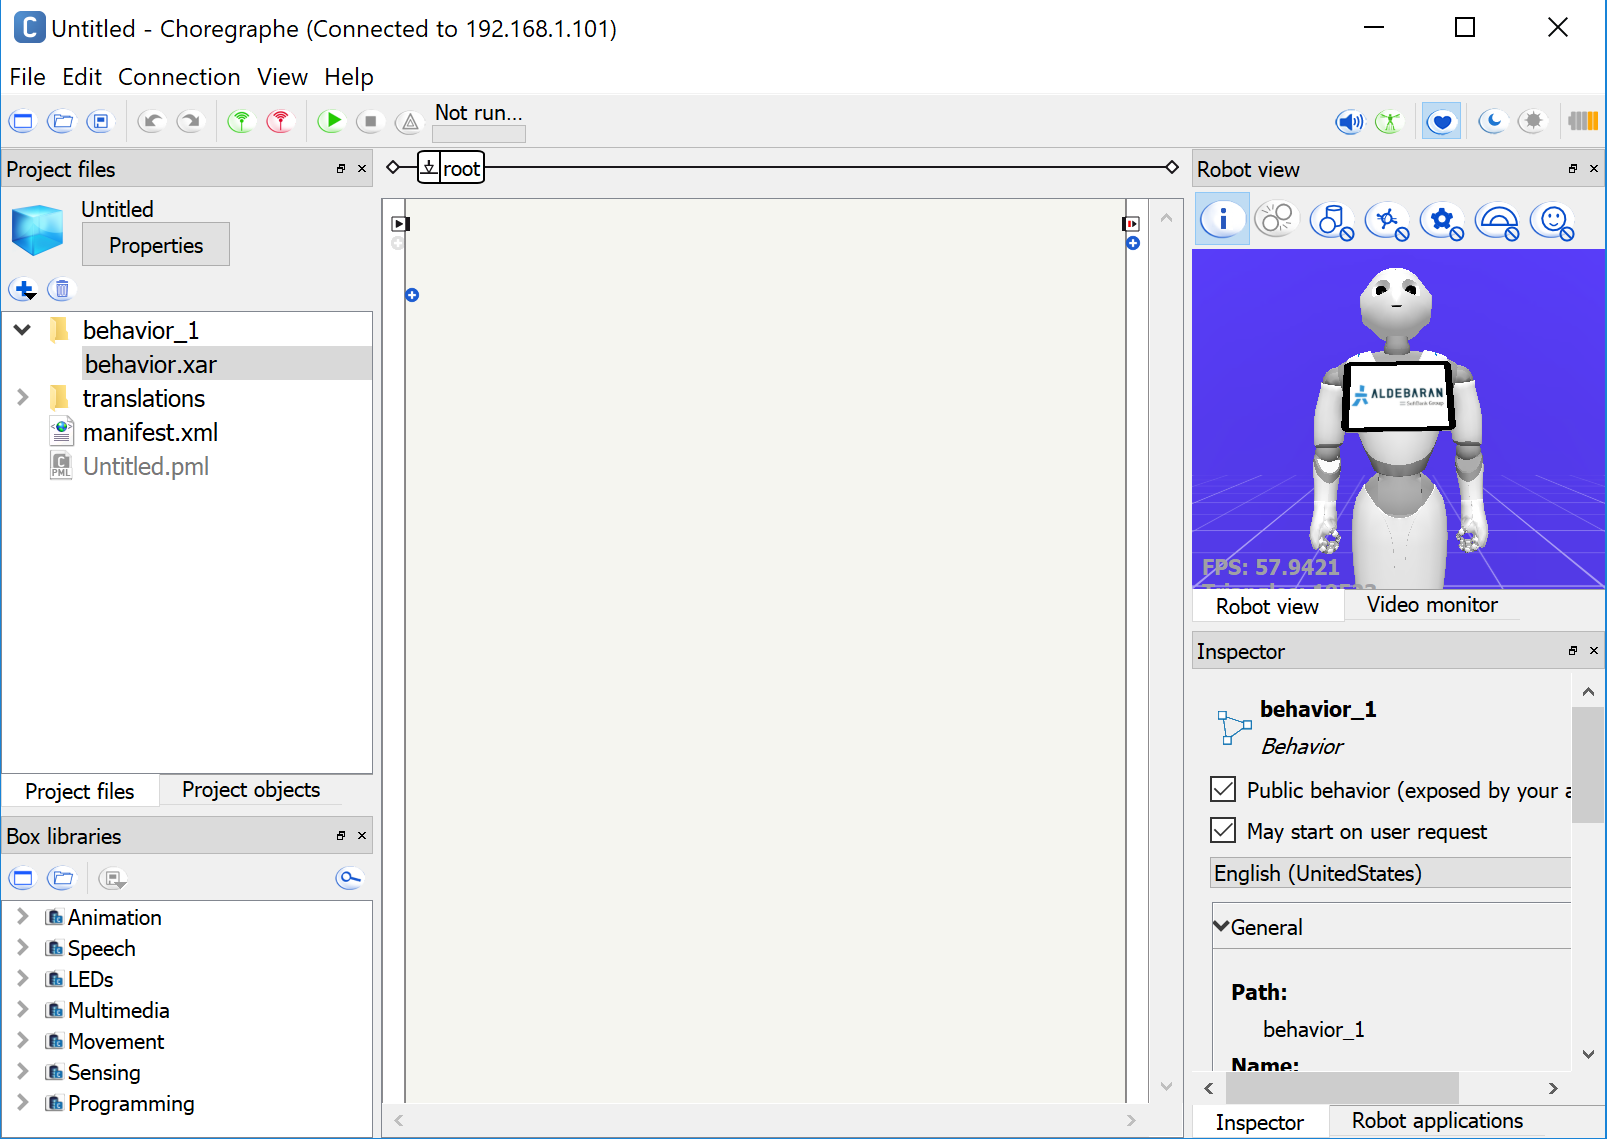
\includegraphics[width=1\textwidth]{immagini/Choregraphe.png}
\caption{Interfaccia del software Aldebaran Choregraphe}
\end{figure}
\vspace{1cm}
Il software si basa su un’architettura di tipo \textit{client-server}, in cui l’interfaccia
utente e l’elaborazione dei comportamenti avvengono su un computer (\textit{client}) e le
istruzioni vengono inviate al robot (\textit{server}) per l’esecuzione.\newline Per comunicare con
il robot, Choregraphe utilizza un protocollo di comunicazione che consente di accedere alle funzionalità
hardware dell'automa, come i sensori, i motori e i moduli di intelligenza artificiale,
attraverso un’API completa e ben documentata. Questo permette agli sviluppatori
di integrare facilmente i comportamenti creati con Choregraphe con altre
applicazioni e sistemi come ad esempio \textit{ROS} (Robot Operating Sistem), framework \textit{open-source} utilizzato per lo sviluppo di applicazioni robotiche.\newline In conclusione, l’intero ambiente di sviluppo si è rivelato essere un potente ed intuitivo
strumento di programmazione visuale facilmente adattabile anche all’ implementazione
di comportamenti più complessi, creando esperienze interattive e coinvolgenti per gli utenti.
}
\newpage

\section{NAOqi OS}
\fontsize{12}{19}\selectfont{
NAOqi OS è un sistema operativo sviluppato da \textit{SoftBank Robotics} per i loro robot umanoidi NAO e Pepper. Si tratta di una distribuzione GNU/Linux basata su Gentoo\footnote{\textbf{Gentoo}: distribuzione Linux basata su sorgenti, che si distingue per il suo approccio altamente personalizzabile e orientato alle prestazioni.} e sviluppata appositamente per le esigenze degli automi dell'azienda \textit{Aldebaran}.
\vspace{1cm}
\begin{figure}[H]
\centering
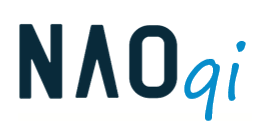
\includegraphics[width=0.48\textwidth]{immagini/naoqi.png}
\caption{Logo di NAOqi OS}
\end{figure}
\vspace{1cm}
La particolarità di questo sistema operativo si ritrova nella sua architettura a componenti modulari. Ogni componente, chiamato "\textit{module}", svolge un compito specifico, come il controllo del movimento, la percezione dei sensori o l'elaborazione del linguaggio naturale.\newline Questi moduli interagiscono tra loro attraverso un sistema di messaggistica per consentire la comunicazione e la cooperazione.\newline NAOqi OS utilizza un middleware chiamato "\textit{ALBroker}" per gestire la comunicazione tra i moduli. L'\textit{ALBroker} funge da intermediario tra i moduli, consentendo loro di pubblicare e sottoscriversi a \textit{topic}, inviare e ricevere messaggi, e richiedere e fornire servizi.
\vspace{0.7cm}
\begin{flushleft}
\textbf{Topic}
\end{flushleft}
Più nello specifico, con \textit{topic} si intende un canale di comunicazione asincrona utilizzato per scambiare messaggi tra i diversi componenti di un sistema robotico.\newline Un topic può essere considerato come un argomento di discussione su cui i nodi del sistema possono pubblicare e sottoscriversi per inviare e ricevere messaggi relativi a quell'argomento specifico.
\begin{figure}[H]
\centering
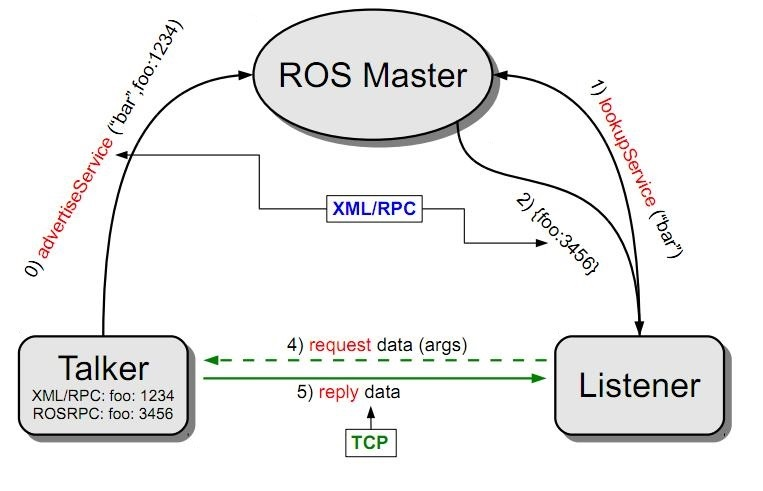
\includegraphics[width=0.88\textwidth]{immagini/comunicazione_ros.png}
\caption{Esempio di comunicazione tra i nodi in ROS}
\end{figure}
\vspace{1cm}
I messaggi possono contenere dati di vario tipo, come informazioni provenienti dai sensori del robot, comandi di controllo, dati di stato, immagini, odometria (consente di stimare e tenere traccia della posizione e dell'orientamento di un robot in base alle informazioni dei suoi motori di movimento) e altro ancora.

 Quando un nodo pubblica un messaggio su un topic, tutti i nodi che si sono sottoscritti a quel topic riceveranno il messaggio e potranno elaborarlo di conseguenza. Ciò consente una comunicazione efficiente e disaccoppiata tra i diversi componenti del sistema robotico, in quanto i nodi possono inviare e ricevere dati senza la necessità di un collegamento diretto uno-a-uno.\vspace{1.5cm}\newline 
 Tornando a NAOqi OS, questo offre una serie di strumenti di sviluppo per facilitare la creazione di applicazioni robotiche. Questi strumenti includono l'ambiente di programmazione visuale Choregraphe, che consente di creare comportamenti per il robot trascinando e rilasciando blocchi di azioni, e l'API di sviluppo NAOqi SDK, che fornisce una vasta gamma di funzioni per interagire con i moduli e controllare il robot.\newline
 \vspace{0.3cm}
 Queste funzioni vengono descritte di seguito:
 \vspace{0.1cm}
 \begin{itemize}
     \item \textbf{Accesso ai sensori}: fornisce un’interfaccia per accedere ai
sensori del robot, come telecamere, microfoni, sensori tattili e giroscopi. Si
possono utilizzare queste informazioni sensoriali per creare comportamenti
basati sulla percezione dell’ambiente circostante.
\vspace{0.5cm}
     \item \textbf{Controllo dei motori}: permette di controllare i motori del robot,
consentendo di gestire il movimento e la postura degli attuatori. Ciò consente
di creare movimenti fluidi e naturali per i robot umanoidi.
\vspace{0.5cm}
     \item \textbf{Gestione del suono}: offre funzionalità per la registrazione e
la riproduzione dei suoni, consentendo ai robot di comunicare e interagire
tramite l’emissione di suoni o la riproduzione di file audio predefiniti.
\vspace{0.5cm}
     \item \textbf{Riconoscimento vocale e linguaggio naturale}: sono inclusi moduli
per il riconoscimento e la sintesi vocale, consentendo ai robot
di comprendere e rispondere ai comandi vocali generando feedback
verbali.
\vspace{0.5cm}
     \item \textbf{Intelligenza artificiale}: sono integrati moduli di intelligenza artificiale,
come il riconoscimento facciale e il riconoscimento degli oggetti, che consentono
ai robot di interagire con gli esseri umani e di analizzare l’ambiente
circostante.
\vspace{0.4cm}
     \item \textbf{Comunicazione}: è supportata la comunicazione tra i robot stessi
o con dispositivi esterni attraverso protocolli come TCP/IP, permettendo
la collaborazione tra più robot o l’integrazione con altri sistemi.
 \end{itemize}
\vspace{1.5cm}
Per concludere, questo sistema operativo embedded\footnote{\textbf{Sistema operativo embedded}: sistema operativo ottimizzato per funzionare su hardware a risorse limitate, con restrizioni di memoria, potenza di calcolo e spazio di archiviazione. Caratterizzato da un basso consumo energetico, affidabilità e una richiesta minima di risorse di sistema rispetto alle distribuzioni \textit{desktop} o \textit{server}.} è progettato per essere multi-piattaforma, per semplificare lo sviluppo di applicazioni robotiche e gestire
comportamenti personalizzati, consentendo agli sviluppatori di concentrarsi
sulla logica dell’applicazione senza doversi preoccupare dei dettagli implementativi
e tecnici di basso livello.
}
\newpage
\end{sloppypar}
\afterpage{\blankpage}